\documentclass[11pt,a4paper,twoside]{article}
\usepackage[portuguese]{babel}
\usepackage{graphicx}  		%% display images
\usepackage{float}			%% make graphics float in place
\usepackage{indentfirst}
\usepackage{hyphenat}
\usepackage{subcaption}		%% allows for subgigures
\usepackage{listings} 		%% for listing code
\usepackage[top=2.50cm, bottom=2.50cm,left=2.50cm, right=2.50cm]{geometry} % margens
\usepackage[colorlinks=true,linkcolor=black,urlcolor=black,bookmarksopen=true]{hyperref} %% Make hyperlinks in index
\usepackage{bookmark} 		% Bookmarks for pdf file
\renewcommand{\baselinestretch}{1.2} 
\usepackage{fancyhdr} 		% creates fancy footers and headers
\pagestyle{fancy}
\lfoot{{\footnotesize Tecnologias de Informação}}
\rfoot{{\footnotesize ESTGA}}
\rhead{Projecto Temático em Desenvolvimento de Aplicações}
\lhead{}

% Title Page
\title{}
\author{}


\begin{document}


\begin{titlepage}
	\centering
	\vfill
	
\includegraphics[width=7cm]{image/ESTGA} % also works with logo.pdf
	\vfill
	
	{\bfseries\Large
		Projeto temático em Desenvolvimento de Aplicações\\
		PyClinic Manual Utilização \\
		\vskip2cm
		%A. Uthor\\
	}    
	
	\vfill
	\textbf{Grupo 5}
	
	António Bento (97737)
	
	Diogo Matos (98017)
	
	Ivan Xavier (92441)
	
	Maykol Santos (74079)
	
	Ricardo Fernandes (49880)
	
	Simão Julião (98045)
	\vfill
\end{titlepage}



\pagenumbering{roman}
\begin{small}
	\tableofcontents
\end{small}

\pagenumbering{roman}
\listoffigures
\newpage\null\thispagestyle{empty}\newpage
\pagenumbering{arabic}



 

\section{Requisitos}
A cliníca que pretenda utilizar este serviço deve possuir um sistema computacional que contenha o sistema operativo Linux ou Windows e ainda uma base de dados SQL na versão 5.7 ou acima.
\section{Atividades Comuns}

Dado que existem funcionalidades comuns às várias profissões presentes na clínica, estas são operadas do mesmo modo entre os mesmos, as atividades referidas são as seguintes:

\begin{itemize}
	\item Aceder ao perfil de utilizador.
	\item Consultar ficha de utente.
	\item Consultar histórico de consultas associadas ao utente.
	\item Consultar histórico de exames associados à consulta.
	
	\item Alterar email de utilizador.
	\item Alterar palavra-passe de utilizador.
\end{itemize}

\subsection{Aceder ao perfil de utilizador.}
Aceder ao perfil de utilizador requer selecionar a aba designada por "Perfil".

\begin{figure}[H]
	\centering
	\includegraphics[width=0.9\linewidth]{image/admin/perfil.png}
	\caption{Perfil do utilizador.}
	\label{fig:perfilutilizador}
\end{figure}

\subsection{Consultar ficha de utente.}
Consultar ficha de utente requer selecionar a aba designada por "Procurar", selecionar o utente pretendido e clicar no botão "Selecionar".

\begin{figure}[H]
	\centering
	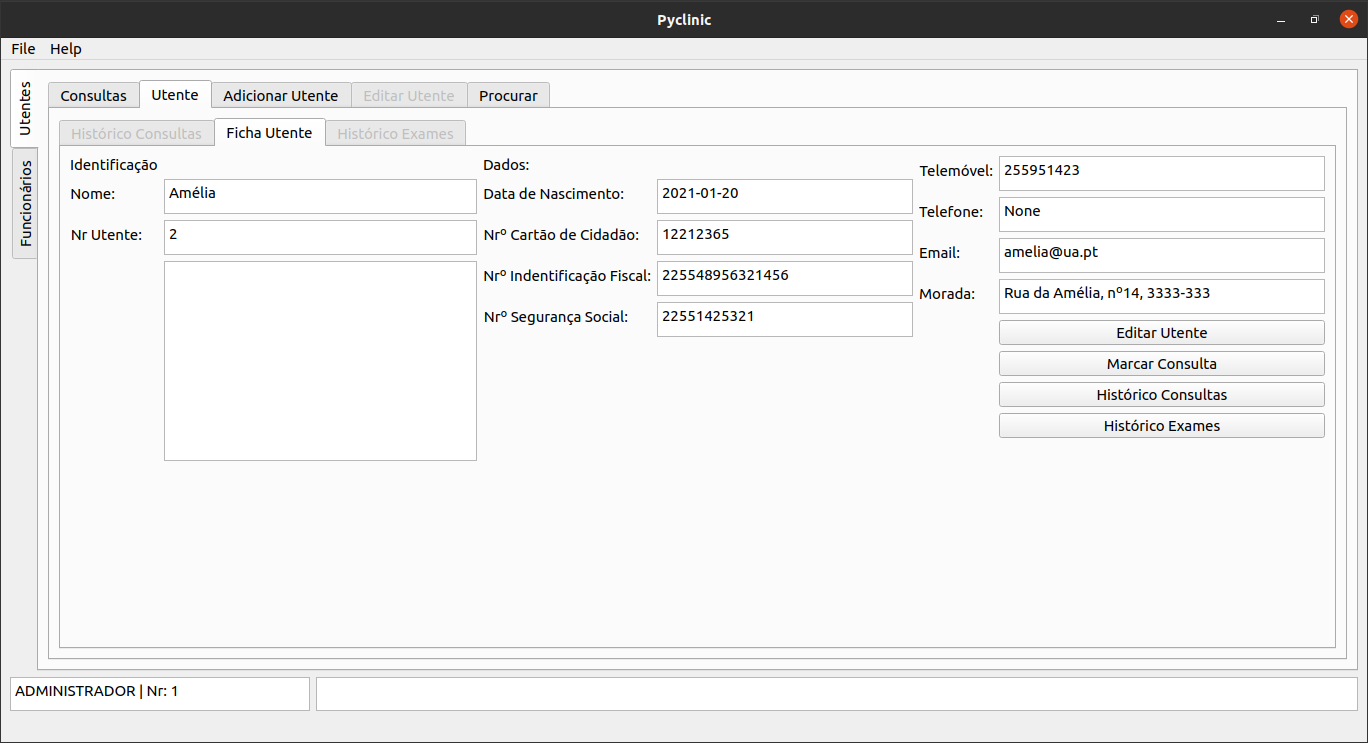
\includegraphics[width=0.9\linewidth]{image/admin/fichaUtente.png}
	\caption{Consultar ficha de utente.}
	\label{fig:fichautente}
\end{figure}

\subsection{Consultar histórico de consultas associadas ao utente.}
Para consultar este histórico é necessário consultar utente e no mesmo ecrã clicar em "Histórico Consultas".

\begin{figure}[H]
	\centering
	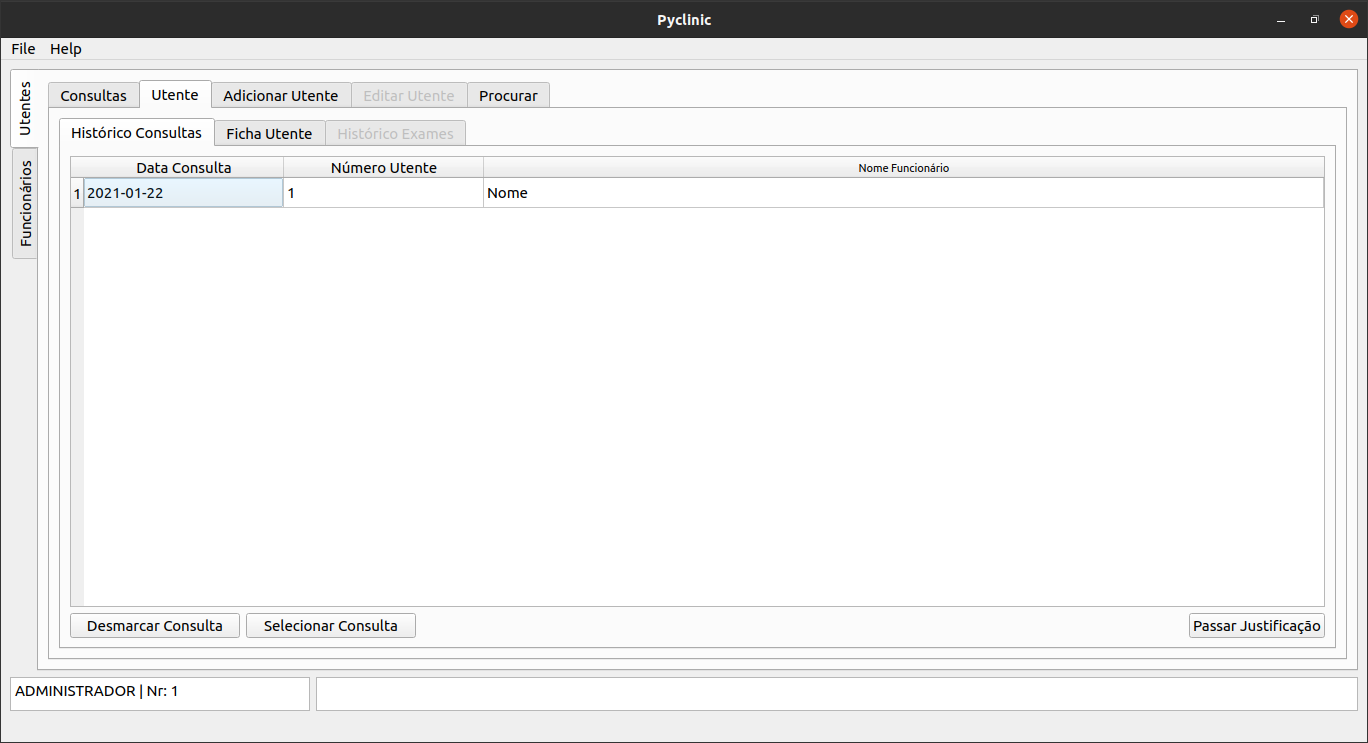
\includegraphics[width=0.9\linewidth]{image/admin/historicoConsultas.png}
	\caption{Consultar histórico Consultas.}
	\label{fig:historicoconsulta}
\end{figure}

\subsection{Consultar histórico de exames associados à consulta.}
Para consultar o histórico de exames é necessário selecionar utente e no ecrã da ficha de utente clicar em "Histórico de Exames".

\begin{figure}[H]
	\centering
	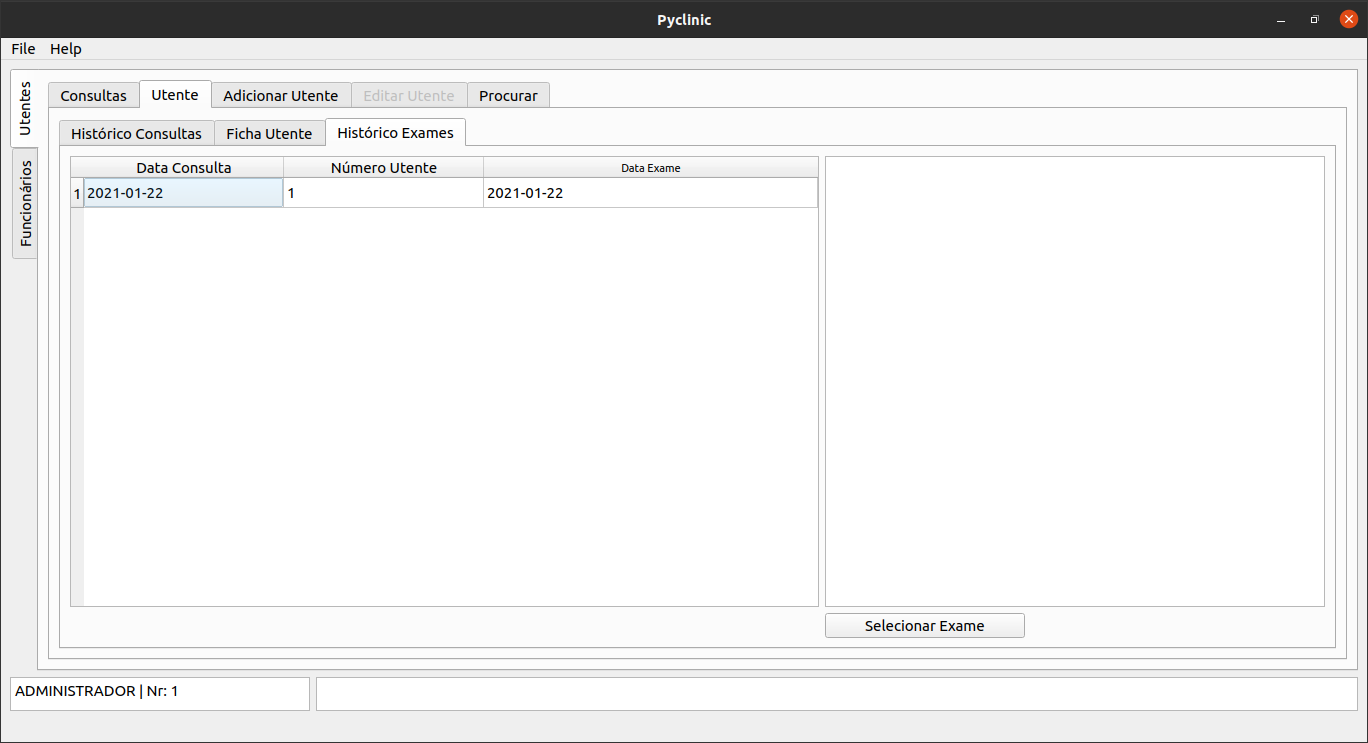
\includegraphics[width=0.9\linewidth]{image/admin/historicoExames.png}
	\caption{Consultar histórico Exames.}
	\label{fig:historicoexame}
\end{figure}

\subsection{Alterar email de utilizador.}
Alterar email de utilizador é possível após aceder ao perfil de utilizador, no qual são alterados os campos designados por "novo email" e se clica em "alterar email".

\begin{figure}[H]
	\centering
	\includegraphics[width=0.9\linewidth]{image/medico/alteraremail.png}
	\caption{Editar e-mail Funcionario.}
	\label{fig:alteraremail}
\end{figure}

\subsection{Alterar palavra-passe de utilizador.}
De modo a alterar a palavra-passe de utilizador é necessário aceder ao perfil de utilizador, preencher os campos denominados por "palavra-passe atual", "palavra-passe nova", "repetir palavra-passe" e clicar em "alterar \textit{password}".

\begin{figure}[H]
	\centering
	\includegraphics[width=0.9\linewidth]{image/medico/alterarpass.png}
	\caption{Editar password Funcionario.}
	\label{fig:alterarpass}
\end{figure}

\section{Médicos}     

Para que o utilizador consiga operar sobre as funcionalidades designadas aos médicos, este terá de efetuar \textit{login} com as credenciais corretas (Nome de utilizador e palavra-passe correspondente), estas presentes na base de dados.

Ao efetuar \textit{login} corretamente, o utilizador adquire a capacidade de:

\begin{itemize}
	\item Consultar histórico de consultas associadas ao médico.
	\item Alterar relatório de consulta.
	\item Alterar prescrição de consulta.
	\item Alterar avisos de consulta.
	\item Adicionar exame.
	\item Consultar exame.
	\item Analisar consulta.
\end{itemize}

\subsection{Consultar histórico de consultas associadas ao médico.}
Consultar histórico de consultas associadas ao médico requer que o utilizador selecione a aba "Consultas", na qual é apresentada a lista de consultas associadas ao médico.

\begin{figure}[H]
	\centering
	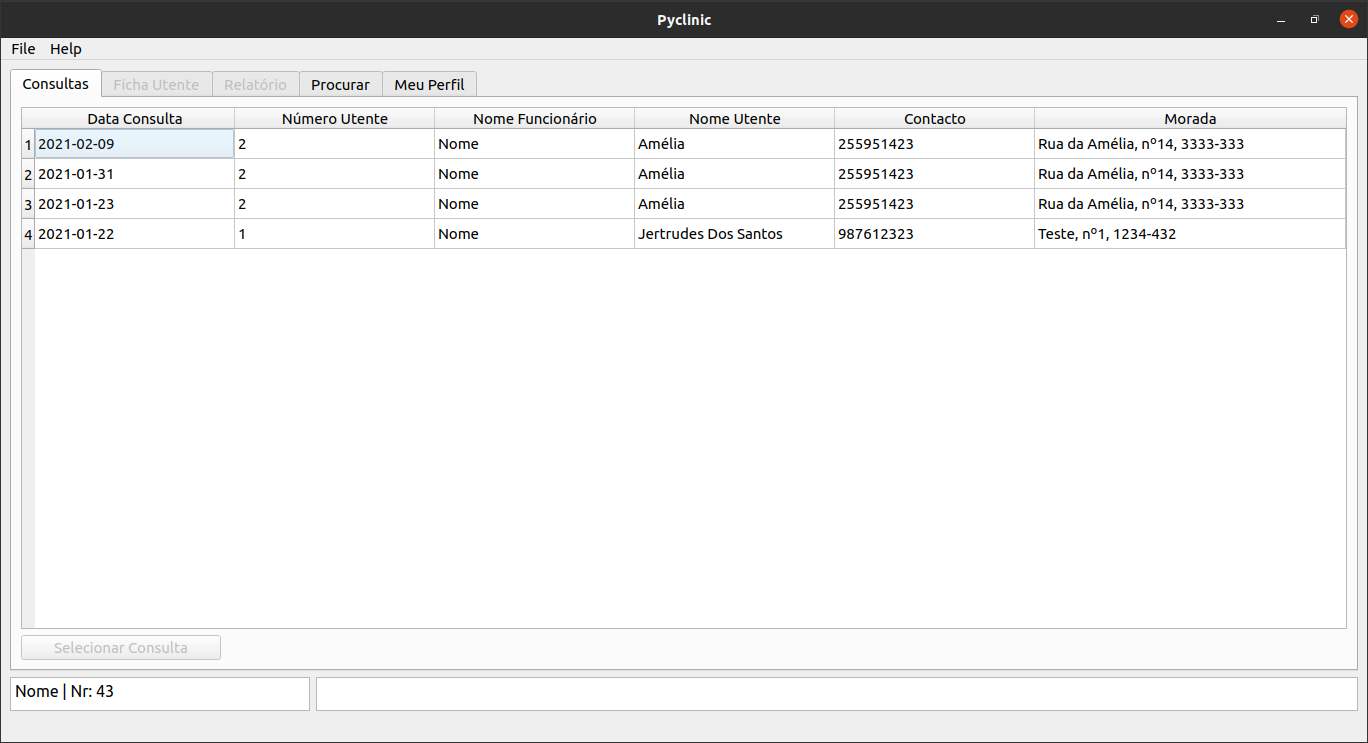
\includegraphics[width=0.9\linewidth]{image/medico/historicoConsultasMedico.png}
	\caption{Histórico de consultas do médico.}
	\label{fig:historicomedico}
\end{figure}

\subsection{Alterar relatório de consulta.}
Alterar relatório de consulta requer que o utilizador selecione a consulta em questão no dia reservado para a mesma, alterando o campo designado por "Relatório" e clicando no botão designado por "Guardar".

\begin{figure}[H]
	\centering
	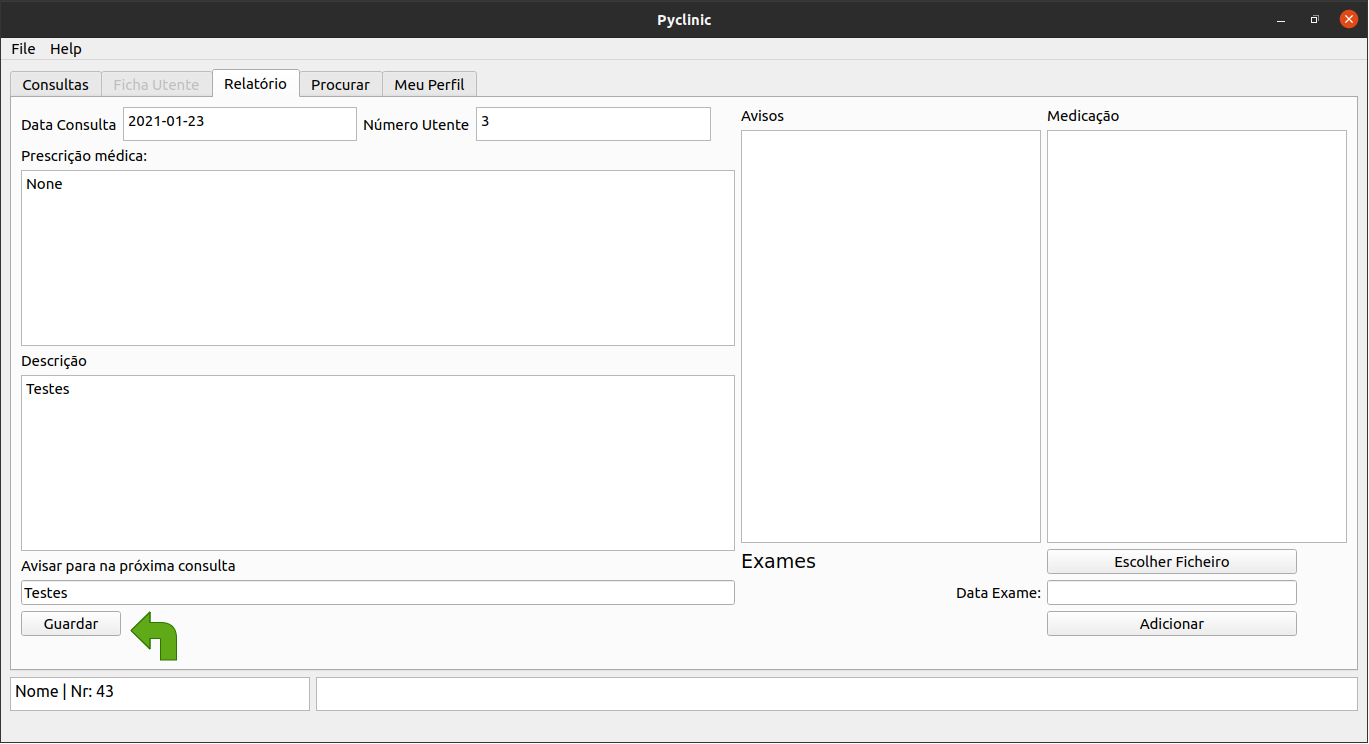
\includegraphics[width=0.9\linewidth]{image/medico/relatorio.png}
	\caption{Editar relatório médico.}
	\label{fig:editarrealtorio}
\end{figure}

\subsection{Alterar avisos de consulta.}
Alterar avisos de consulta requer ser efetuado no mesmo dia que a consulta em questão, em seguida selecionar consulta, no ecrã atual registar os avisos no espaço designado por "Avisos" e clicar em "Guardar".

\begin{figure}[H]
	\centering
	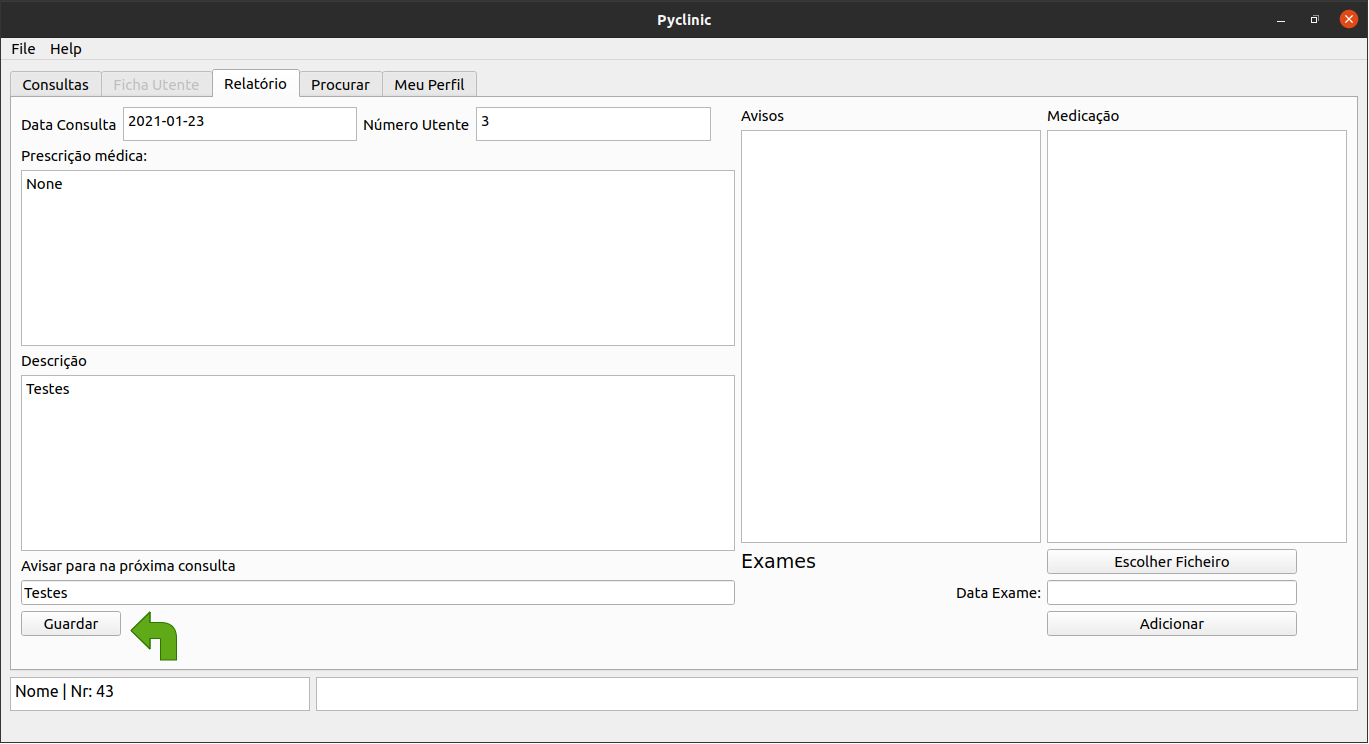
\includegraphics[width=0.9\linewidth]{image/medico/relatorio.png}
	\caption{Editar aviso de consulta.}
	\label{fig:editaraviso}
\end{figure}

\subsection{Adicionar exame.}
Adicionar exame requer que o utilizador selecione a consulta na aba "Consultas", selecionar a aba "Relatório", em seguida deve clicar no botão "Escolher Ficheiro" e selecionar o exame, para confirmar o envio deve clicar no botão "Adicionar".

\begin{figure}[H]
	\centering
	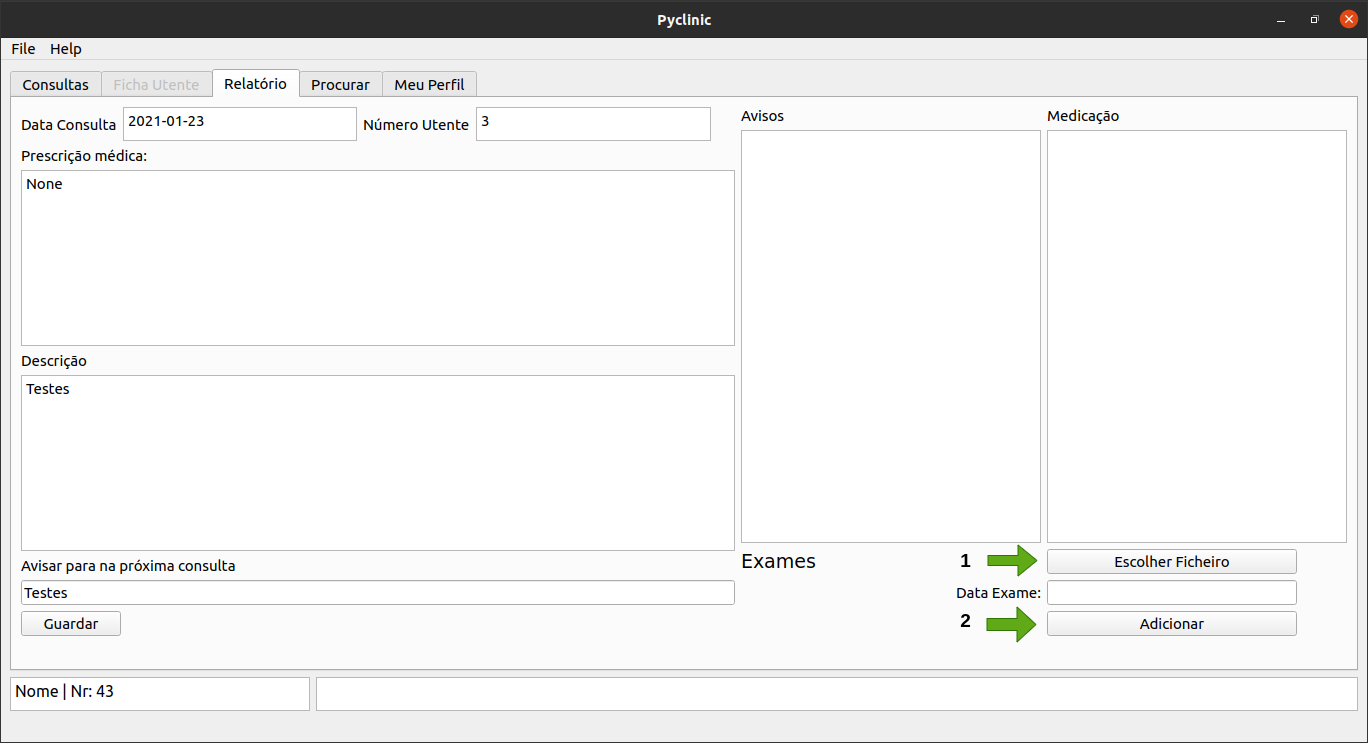
\includegraphics[width=0.9\linewidth]{image/medico/exames.png}
	\caption{Adicionar Exame.}
	\label{fig:adicionarexame}
\end{figure}

\subsection{Consultar exame.}
Consultar exame requer que o utilizador selecione o utente na aba "Procurar", na qual será encaminhado para a aba "Ficha de Utente", em seguida deve clicar no botão "Histórico de Exames" e selecionar o exame na tabela, para confirmar deve clicar no botão "Selecionar Exame".

\begin{figure}[H]
	\centering
	\includegraphics[width=0.9\linewidth]{image/medico/ConsultarExame.png}
	\caption{Consultar Exame.}
	\label{fig:consultarexame}
\end{figure}

\subsection{Analisar consulta.}
De modo a analisar uma consulta é necessário ou aceder ao histórico de consultas associadas ao médico, ou associadas ao utente e clicar em "Selecionar Consulta".\\

\begin{figure}[H]
	\centering
	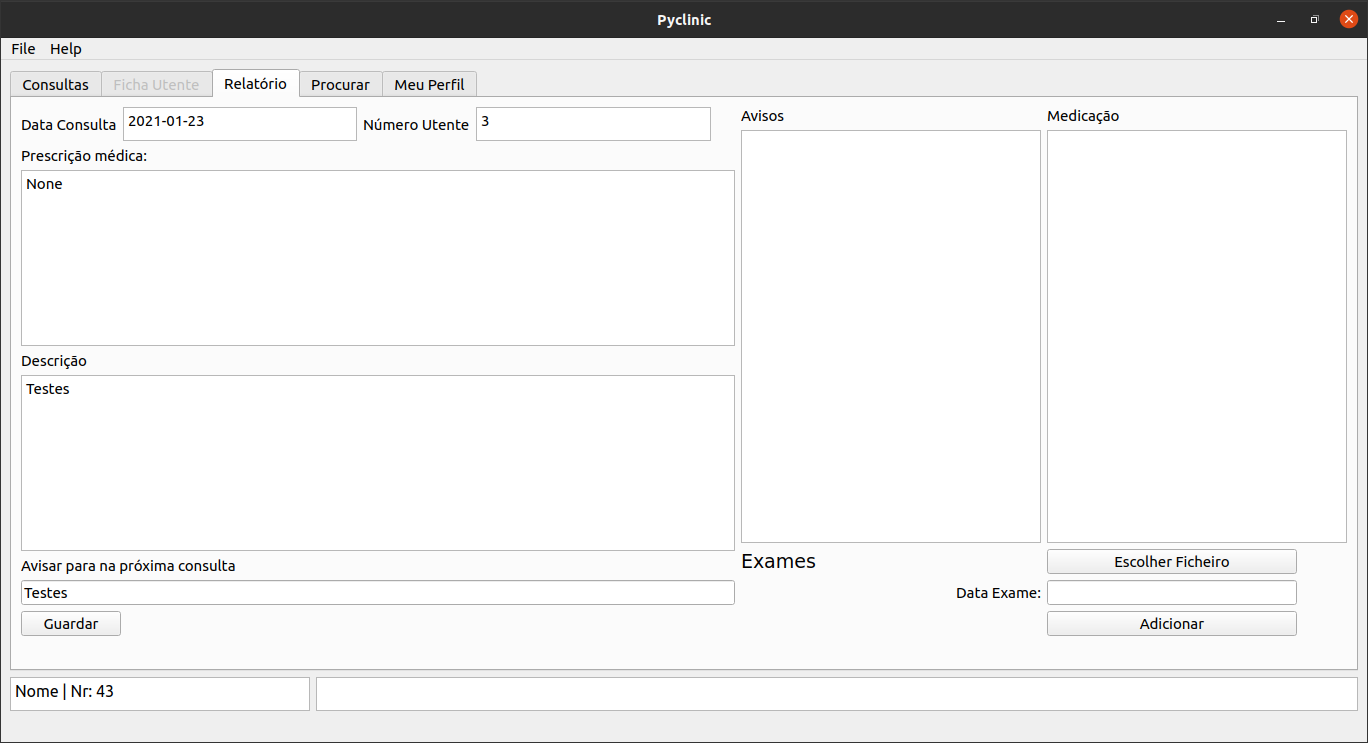
\includegraphics[width=0.9\linewidth]{image/medico/relatorio1.png}
	\caption{observar Consulta.}
	\label{fig:verconsulta}
\end{figure}

Para além das referidas, os médicos são capazes das seguintes funcionalidades comuns:

\begin{itemize}
	\item Aceder ao perfil de utilizador.
	\item Consultar utentes.
	\item Consultar histórico de consultas associadas ao utente.
	\item Consultar histórico de exames associados à consulta.
	\item Adicionar exame.
	\item Analisar consulta.
	\item Alterar email de utilizador.
	\item Alterar palavra-passe de utilizador.
\end{itemize}


\section{Enfermeiros}
	
	Grande parte das funcionalidades de enfermeiro ou são comuns ou são partilhadas com o médico, à exceção de administrar medicação que é particular aos enfermeiros.
	
	Para realizar qualquer atividade o enfermeiro tem de entrar no sistema com as respetivas credenciais.
	
	Registar medicação administrada requer que o dia da consulta seja o mesmo aquando realização desta tarefa, com isto é necessário selecionar a consulta, alterar o campo indicado como "Medicação Administrada" e clicar em "Guardar".
	
	O enfermeiro é também capaz das seguintes operações:
	
	\begin{itemize}
		\item Aceder ao perfil de utilizador.
		\item Consultar utentes.
		\item Consultar histórico de consultas associadas ao utente.
		\item Consultar histórico de exames associados à consulta.
		\item Alterar email de utilizador.
		\item Alterar palavra-passe de utilizador.
	\end{itemize}
	
	Tal como o médico, o enfermeiro é capaz de:
	
	\begin{itemize}
		\item Analisar consulta.
	\end{itemize}
	

\section{Rececionista}

Os rececionistas são capazes das seguintes funcionalidades:

\begin{itemize}
	\item Editar ficha de utente.
	\item Adicionar utente.
	\item Agendar consulta.
	\item Desativar utente.
	\item Desmarcar Consulta
\end{itemize}

\subsection{Editar ficha de utente.}
Para editar a ficha de utente primeiro é necessário consultar a ficha do mesmo em questão e no ecrã atual clicar em "Editar utente", após a mudança de ecrã o utilizador deverá alterar os campos necessários e clicar em "Editar utente". 

\begin{figure}[H]
	\centering
	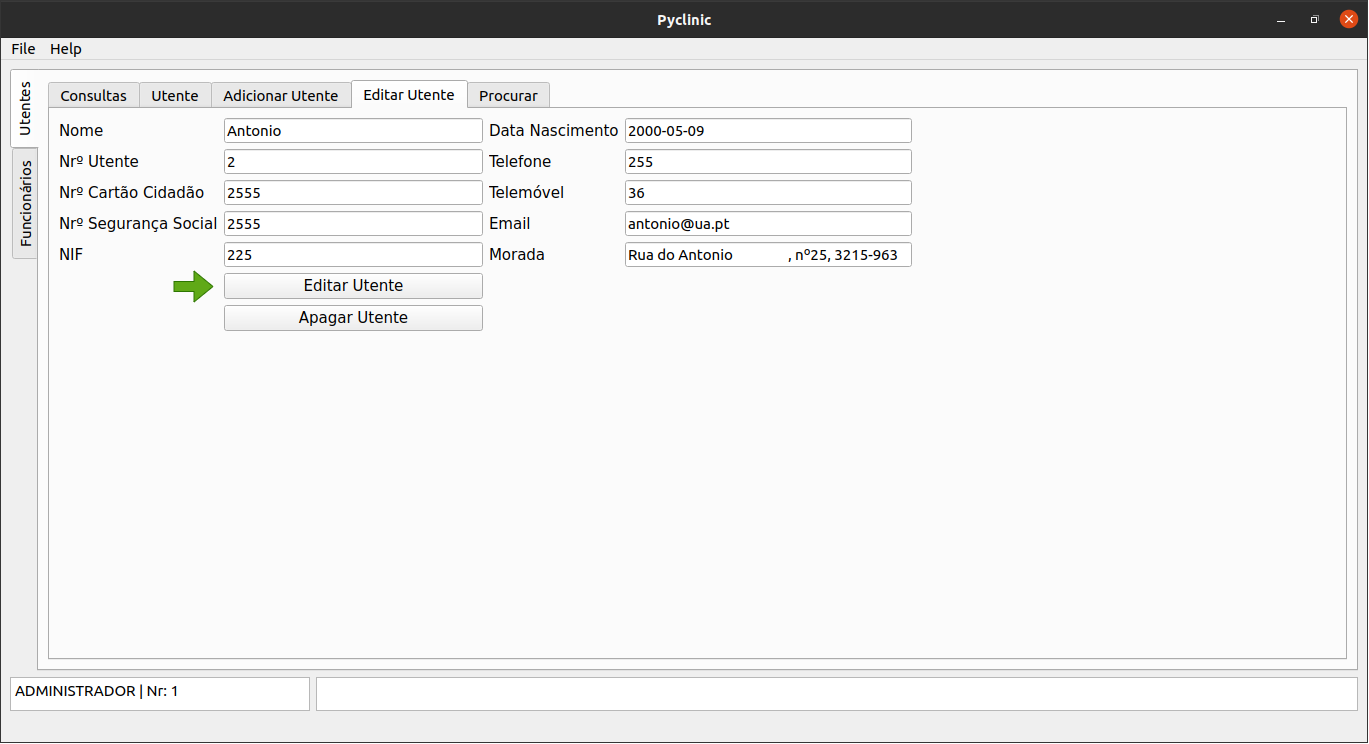
\includegraphics[width=0.9\linewidth]{image/rececionista/editarUtente.png}
	\caption{Editar dados Utentes.}
	\label{fig:editarutente}
\end{figure}

\subsection{Adicionar utente.}
Adicionar utentes deve ser realizado na aba "Adicionar utente", neste ecrã o utilizador deverá preencher os dados de utente corretamente e clicar em "Adicionar". 

Nota: Para as tarefas 1 e 2, a data de nascimento deverá respeitar o seguinte formato AAAA-MM-DD.

\begin{figure}[H]
	\centering
	\includegraphics[width=0.9\linewidth]{image/rececionista/adicionarutente.png}
	\caption{Adicionar utentes.}
	\label{fig:adicionarutente}
\end{figure}

%\begin{figure}[H]
%	\centering
%	\includegraphics[width=0.9\linewidth]{image/rececionista/perfil.png}
%	\caption{Editar password Funcionario.}
%	\label{fig:adicionarutente}
%\end{figure}

\subsection{Agendar consulta.}
Para ser possível agendar uma consulta deve ser selecionado um utente na tabela de pesquisa principal, de seguida na ficha do mesmo deve ser selecionada a opção 'Confirmar Marcação' depois devem ser preenchidos os campos corretamente, deve ainda ser selecionada uma data e hora disponíveis e confirmada a marcação de consulta.

\begin{figure}[H]
	\centering
	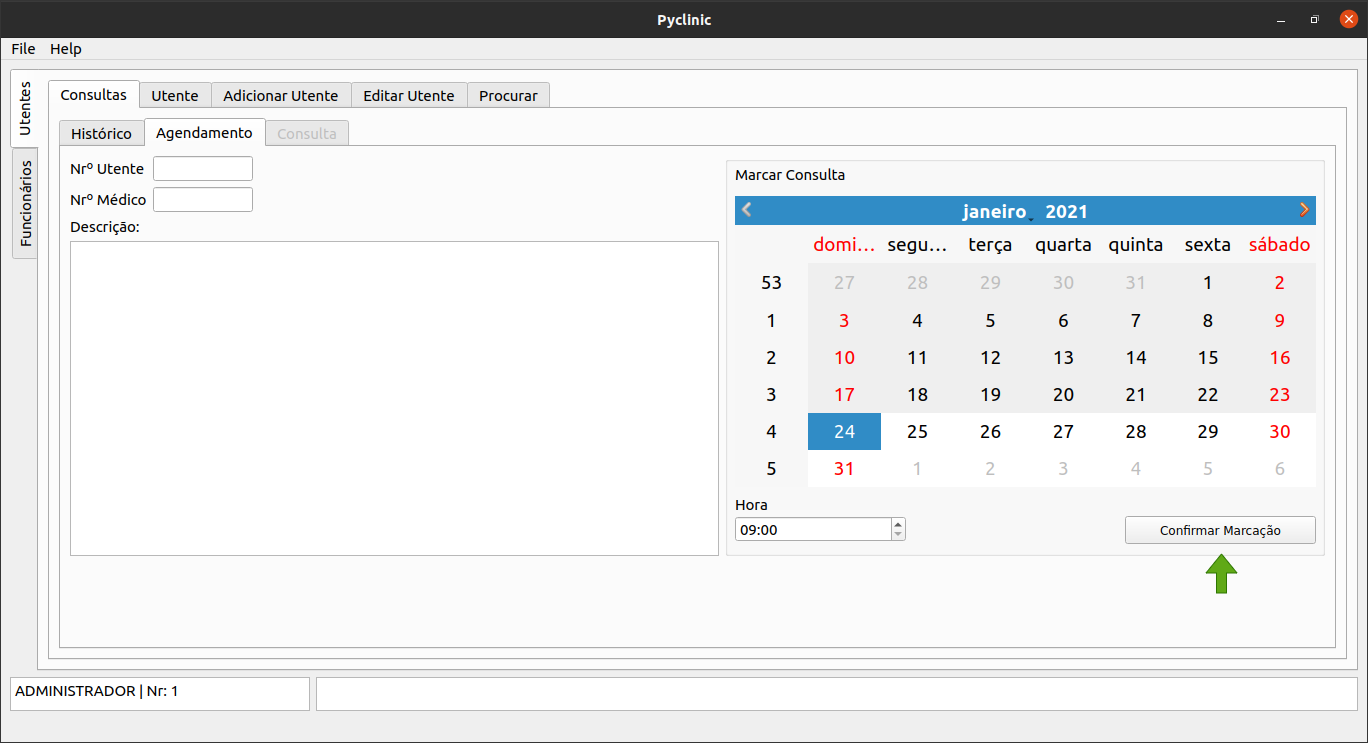
\includegraphics[width=0.9\linewidth]{image/rececionista/marcarConsulta.png}
	\caption{Marcação Consulta.}
	\label{fig:marcarconsulta}
\end{figure}

\subsection{Desativar utente.}
Desativar utente deve ser realizado na ficha do mesmo ao clicar em "Apagar utente".

\begin{figure}[H]
	\centering
	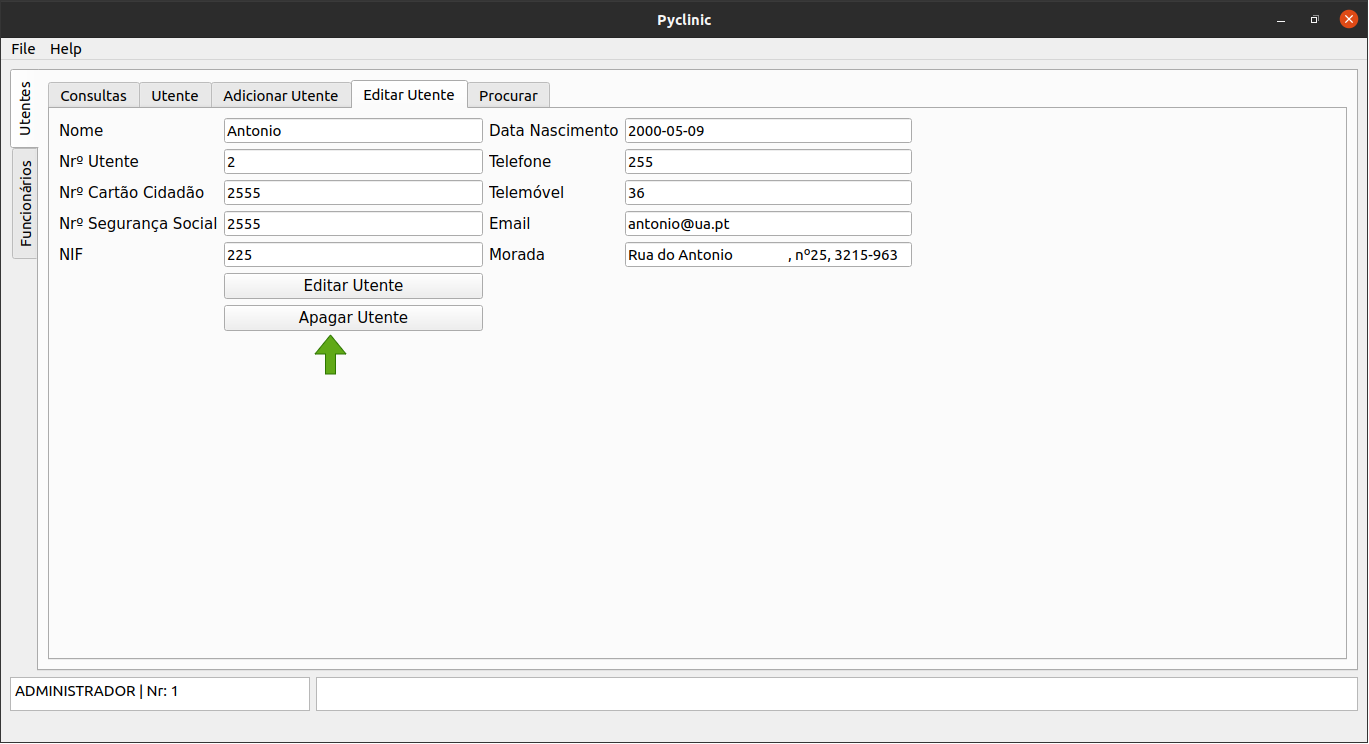
\includegraphics[width=0.9\linewidth]{image/rececionista/apagarUtente.png}
	\caption{Desativar Utente.}
	\label{fig:desativarUtente}
\end{figure}

\subsection{Desmarcar Consulta}
Para desmarcar uma consulta o rececionista deve aceder ao histórico de consultas do utente atravé da sua ficha e de seguida selecionar a consulta que deseja desmarcar e selcionar o botão 'Desmarcar Consulta'.

\begin{figure}[H]
	\centering
	\includegraphics[width=0.9\linewidth]{image/rececionista/desmarcarconsulta.png}
	\caption{Desmarcar Consulta.}
	\label{fig:desmarcarconsulta}
\end{figure}

\section{Administrador}

O administrador para além de ser capaz de todas as funcionalidades referidas anteriormente, possui algumas funcionalidades específicas ao mesmo, tais como:

\begin{itemize}
	\item Adicionar funcionário.
	\item Editar funcionário.
	\item Eliminar funcionário.
\end{itemize}

\subsection{Adicionar funcionário.}
Para adicionar funcionário o utilizador deve aceder à aba "Adicionar Funcionário", preencher todos os campos necessários e de seguida clicar em "Adicionar".

\begin{figure}[H]
	\centering
	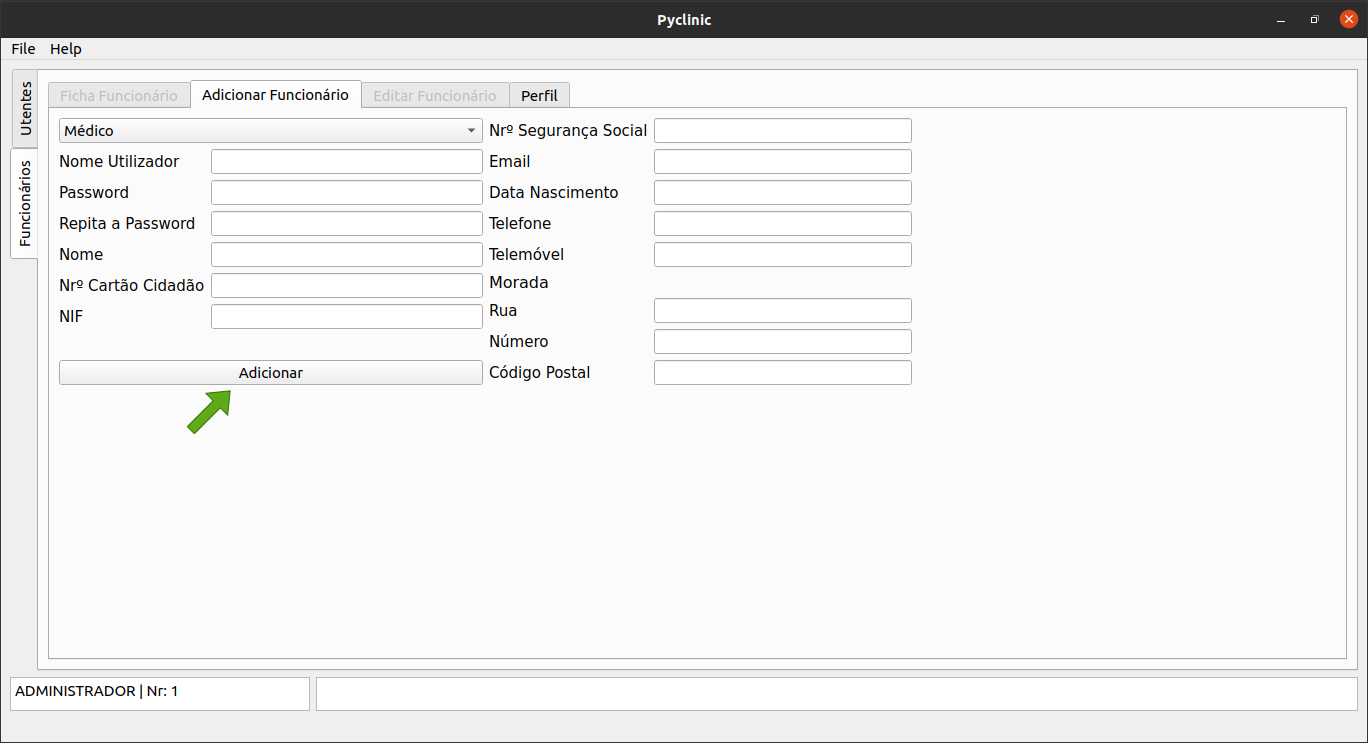
\includegraphics[width=0.9\linewidth]{image/admin/adicionarFuncionario.png}
	\caption{Adicionar Funcionário.}
	\label{fig:adicionarfuncionario}
\end{figure}

\subsection{Editar funcionário.}
Para editar um funcionário o utilizador deve aceder à aba "Procurar" e no campo "Tipo de Procurar:" e selecionar "Funcionário", o utilizador deve selecionar na tabela o funcionário que pretende editar e confirmar no botão "Selecionar", em seguida deve clicar no botão "Editar Funcionário" que se encontra dentro da aba "Ficha de Funcionário", na aba "Editar Funcionário" pode alterar os campos pretendidos e de seguida clicar em "Editar Funcionário" para confirmar a edição.

\begin{figure}[H]
	\centering
	\includegraphics[width=0.9\linewidth]{image/admin/EditarFuncionario.png}
	\caption{Editar Funcionário.}
	\label{fig:editarfuncionario}
\end{figure}

\subsection{Eliminar funcionário.}
Para eliminar um funcionário o utilizador deve aceder à aba "Procurar" e no campo "Tipo de Procurar:" e selecionar "Funcionário", o utilizador deve selecionar na tabela o funcionário que pretende editar e confirmar no botão "Selecionar", em seguida deve clicar no botão "Editar Funcionário" que se encontra dentro da aba "Ficha de Funcionário", na aba "Editar Funcionário" clique no botão "Apagar Funcionário".

\begin{figure}[H]
	\centering
	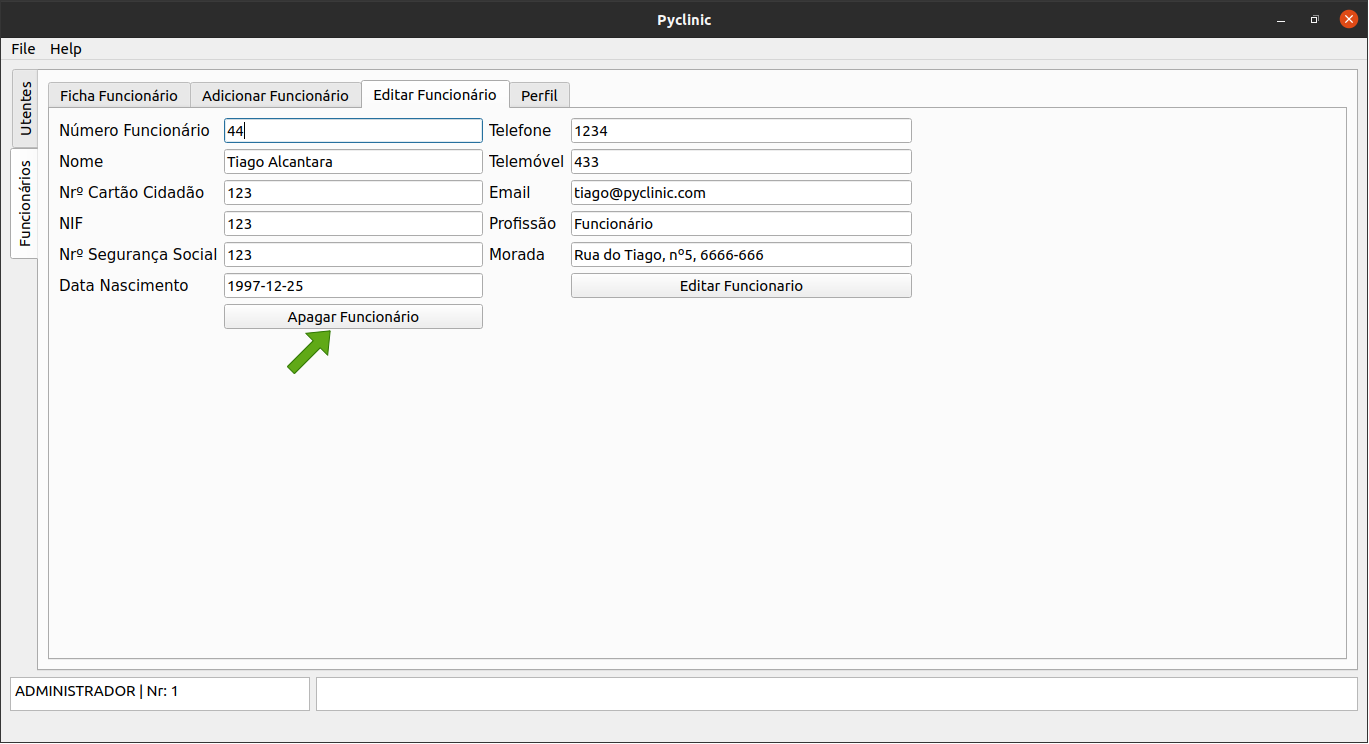
\includegraphics[width=0.9\linewidth]{image/admin/apagarFuncionario.png}
	\caption{Eliminar Funcionário.}
	\label{fig:eliminarfuncionario}
\end{figure}

\end{document}  

  